\section{Methodology}\label{sec:methodology}
\textit{We will write an introduction to the methodology section here, as well as add more subsections in the future. Below is the first subsection describing the data normalization process and the reasons for choosing to only do Norm 3. Please let us know if the explanation and mathematical notation is clear.}

\subsection{Evaluation Metrics}
To evaluate the performance of our models in predicting major oxide compositions from \gls{libs} data, we will use two key metrics: \gls{rmse} and standard deviation of prediction errors.

\gls{rmse} will be used as a measure of accuracy, quantifying the difference between the predicted and actual values of the major oxides in the samples. It is defined by the equation:

\begin{equation}
    RMSE = \sqrt{\frac{1}{n} \sum_{i=1}^{n} (y_i - \hat{y}_i)^2},
\end{equation}

where $y_i$ represents the actual values, $\hat{y}_i$ the predicted values, and $n$ the number of observations. A lower RMSE indicates better accuracy.

To assess the robustness of our models, we will consider the standard deviation of prediction errors across each oxide and test instance. This metric measures the variability of the prediction errors and provides insight into the consistency of the model's performance. It is defined as:

\begin{equation}
    \sigma_{error} = \sqrt{\frac{1}{n-1} \sum_{i=1}^{n} (e_i - \bar{e})^2},
\end{equation}

where $e_i = y_i - \hat{y}_i$ and $\bar{e}$ is the mean error. A lower standard deviation indicates better robustness.

By using these two metrics, we aim to comprehensively evaluate the performance of our models in terms of both accuracy and robustness, which are crucial for the reliable prediction of major oxide compositions from \gls{libs} data.

\subsection{Data Normalization}
The \gls{chemcam} instrument consists of three spectrometers, each producing 2048 channels.
For data normalization, we follow the approach taken by the SuperCam team and normalize across individual spectrometers' wavelength ranges, known as Norm 3~\cite{andersonPostlandingMajorElement2022}.
This method ensures that each spectrometer's data is normalized independently.

Intuitively, Norm 3 can be understood as follows: for each sample, we consider the data from each spectrometer separately. Within each spectrometer, we divide the intensity of each channel by the sum of all channel intensities for that spectrometer. This process is repeated for all three spectrometers, resulting in normalized data that preserves the relative intensities within each spectrometer while allowing for comparisons across different samples.
Figure~\ref{fig:spectral_plot} shows a spectral plot of the \gls{ccs} data for the \textit{ultramafic} sample, illustrating the three distinct spectral regions, each captured by one of the three spectrometers. Specifically, one spectrometer captures the \gls{uv} region, another captures the \gls{vio} region, and the third captures the \gls{vnir} region.

\begin{figure}[H]
	\centering
	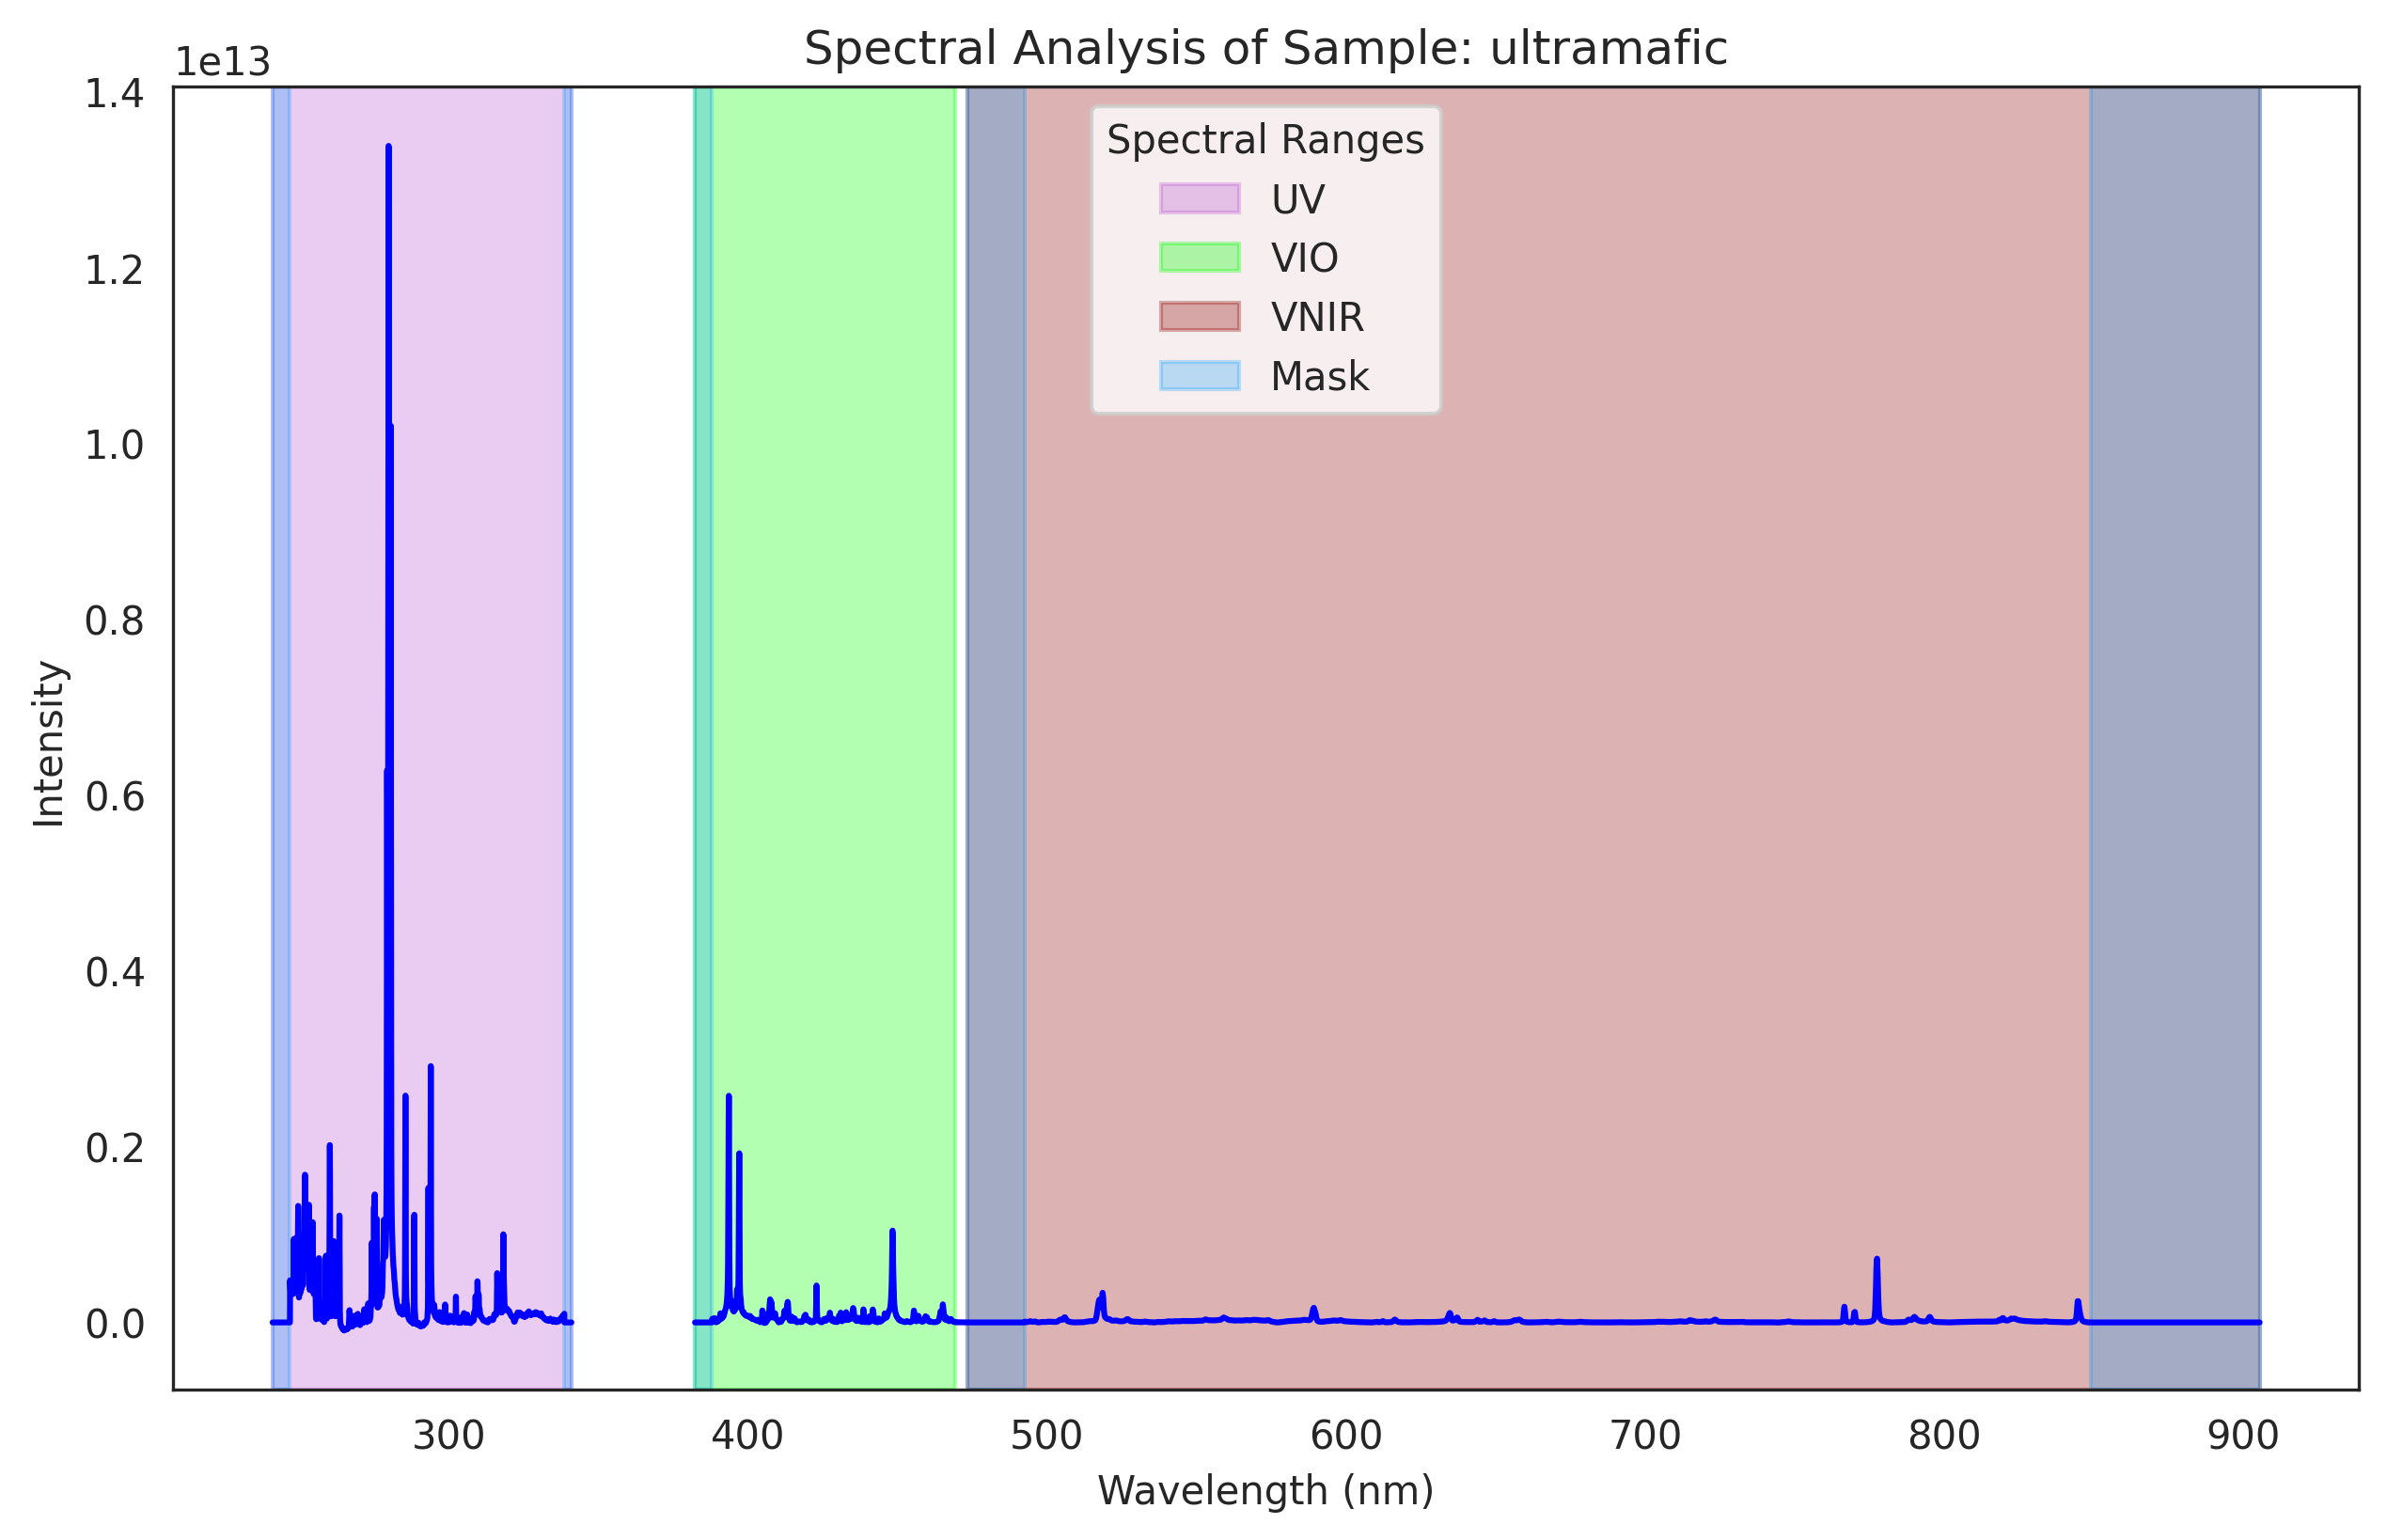
\includegraphics[width=0.5\textwidth]{images/spectral_plot.png}
	\caption{Spectral plot of the \gls{ccs} data for the \textit{ultramafic} sample. The wavelengths represent the spectral channels.}
	\label{fig:spectral_plot}
\end{figure}

Formally, Norm 3 is defined as:

\begin{equation}
	\tilde{X}_{i,j}^{(s)} = \frac{X_{i,j}^{(s)}}{\sum_{j=1}^{N} X_{i,j}^{(s)}},
\end{equation}

where:

\begin{itemize}
	\item $\tilde{X}_{i,j}^{(s)}$ is the normalized wavelength intensity for the $i$-th sample in the $j$-th channel on the $s$-th spectrometer.
	\item $X_{i,j}^{(s)}$ is the original wavelength intensity for the $i$-th sample in the $j$-th channel on the $s$-th spectrometer.
	\item $N = 2048$ is the number of channels in each spectrometer.
	\item $s \in \{1, 2, 3\}$ is the index of the spectrometer.
\end{itemize}

This normalization method results in a total of $3N = 6144$ normalized features for each sample, as each of the three spectrometers contributes 2048 channels.
